\chapter{はじめに}

\section{研究の背景}
当研究室では飛行ロボットコンテストに出場するために飛行機の設計・製作を行っている.今年度は一般部門に出場するために固定翼の作成と、マルチコプター部門に出場するためにマルチコプターの製作を行った.固定翼の部品はアクリルを用いておりレーザ加工を行い制作されている.(図\ref{fig:acril})レーザ加工を用いる事によって部品加工時間が短縮され、また部品の大量生産を可能にした.また同じようにマルチコプターの胴体の部分をレーザ加工で加工してあるためこちらも大量生産・製作時間の短縮を実現している.(図\ref{fig:doutai}).以上の製作方法を用いて機体を制作した後、プログラムなど制御関係を終わらし大会参加を行い決勝でよい成績を残す事が目的となっている.大会には出場出来たものの決勝には進出することが出来ず予選敗退だった。敗退の要因であった縦安定についてストロー飛行機製作を通して学ぼうと考えた.
\begin{figure}[htbp]
  \begin{center}
    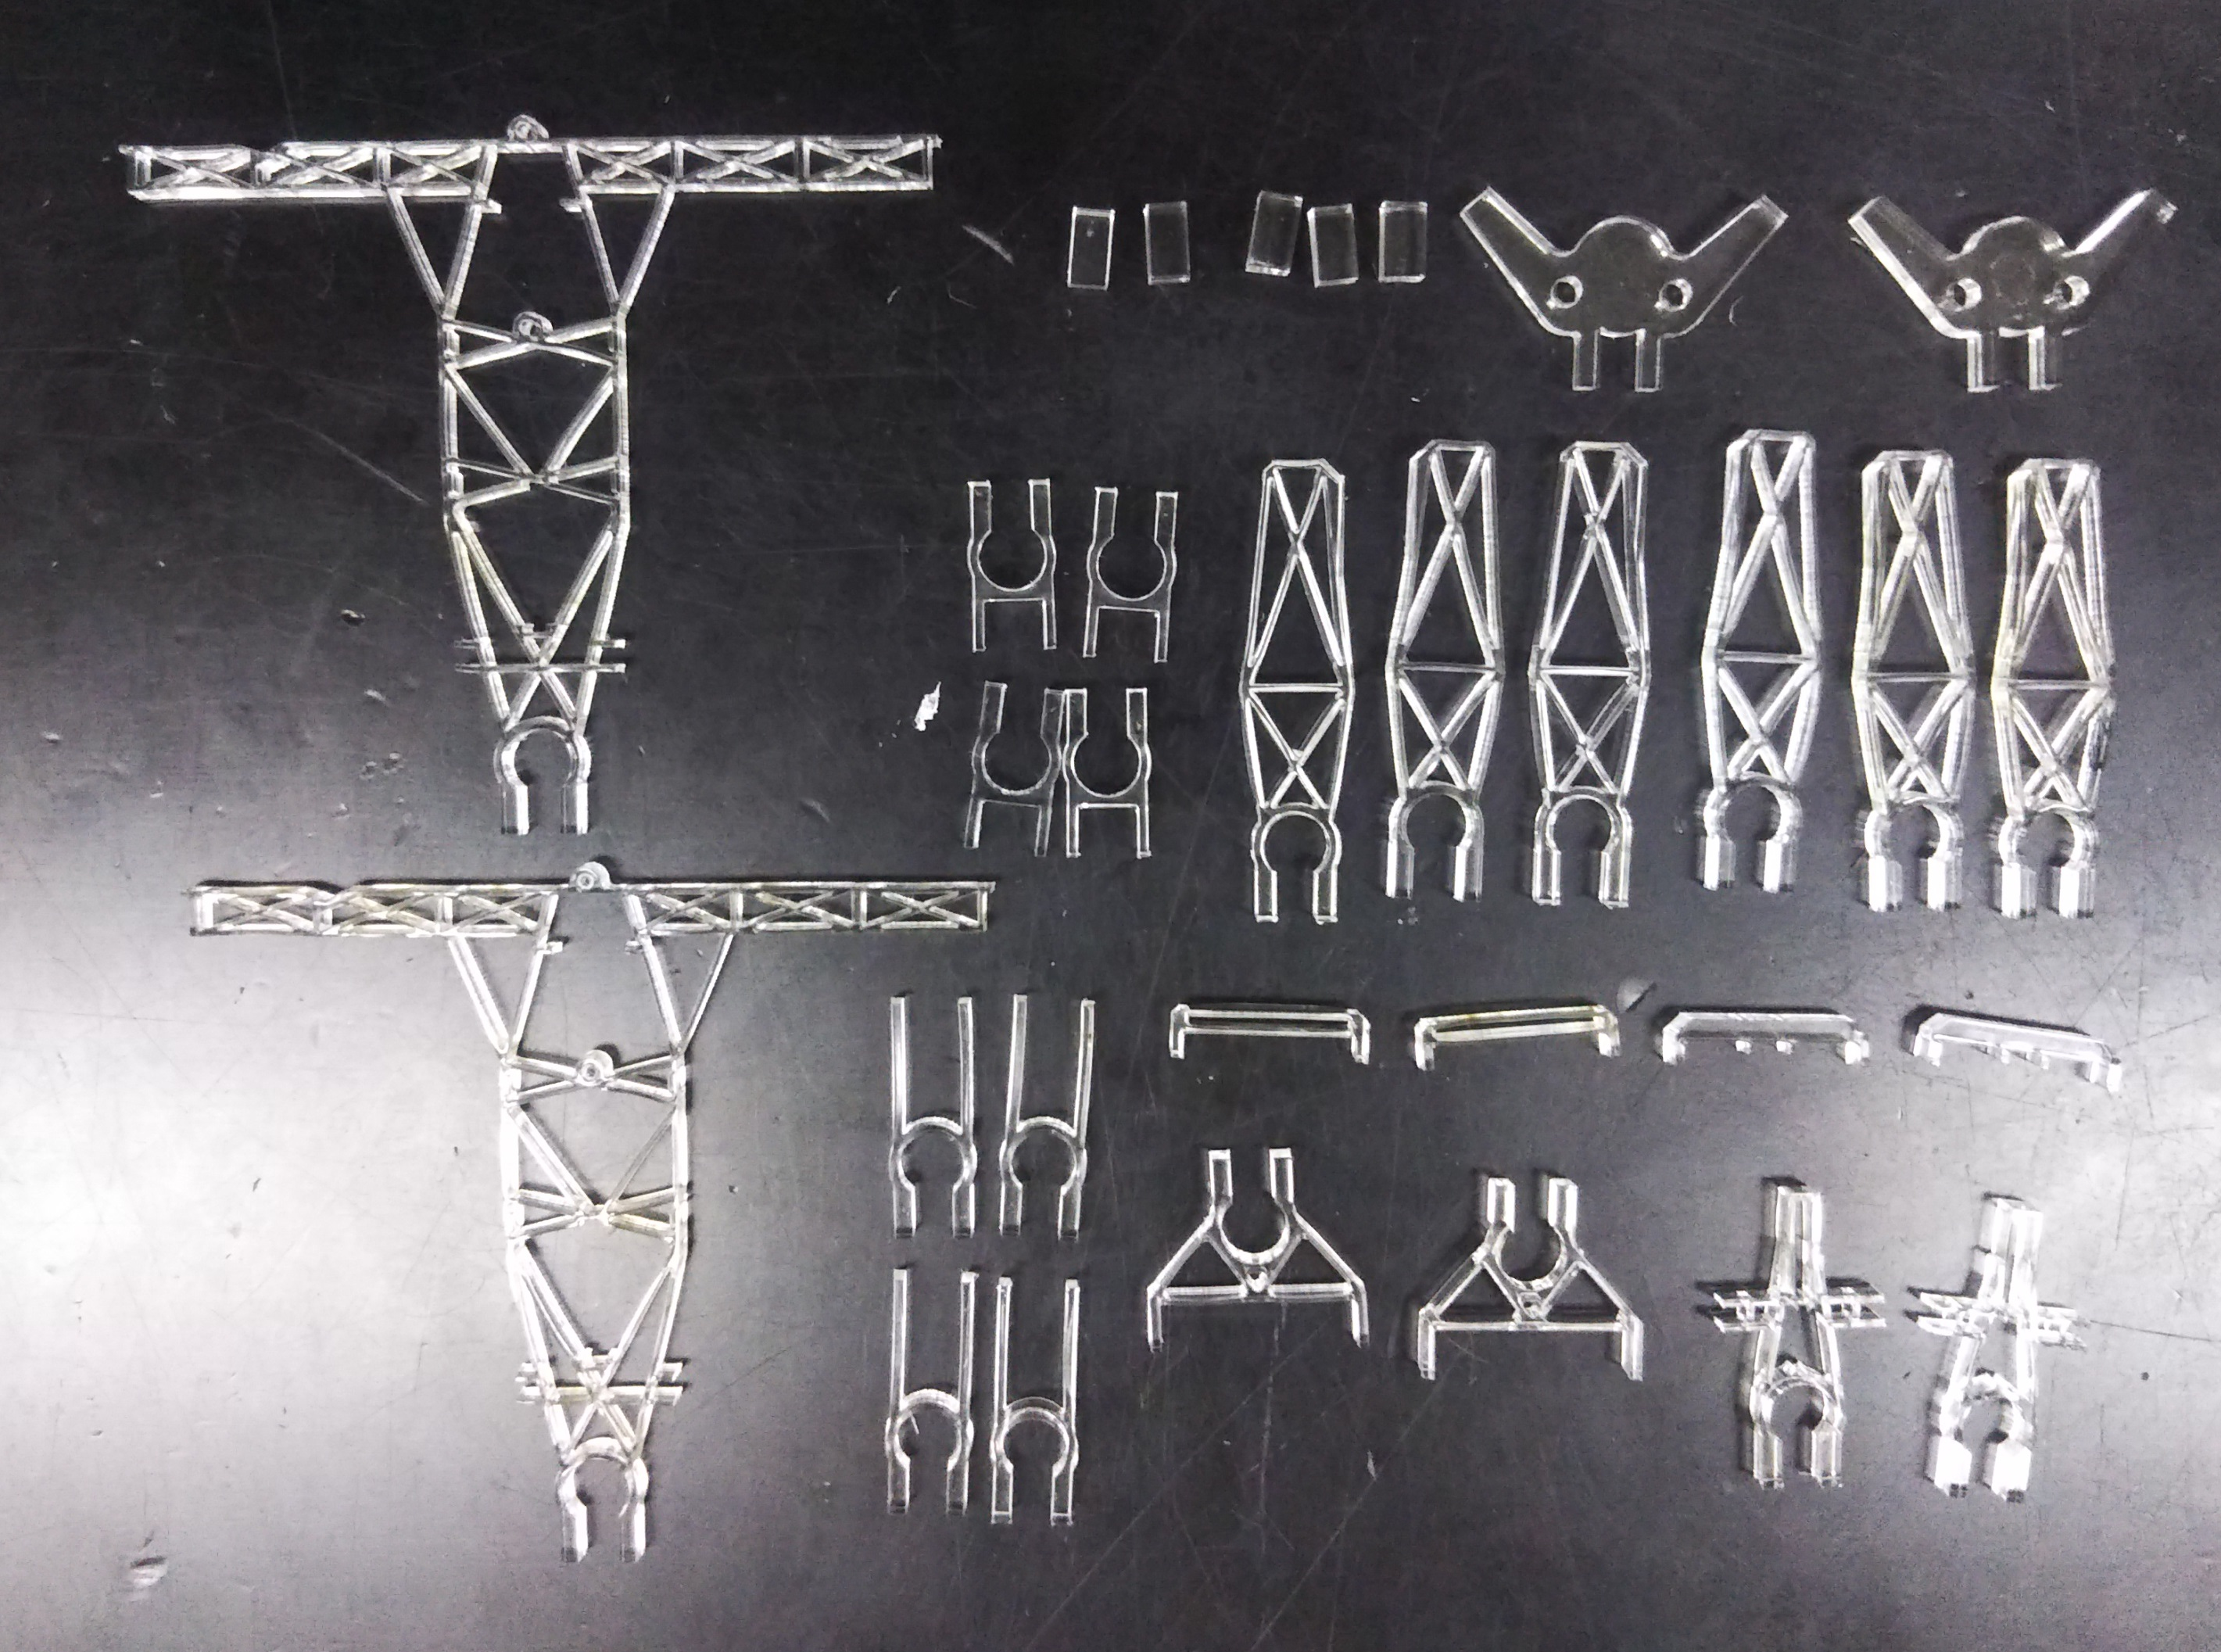
\includegraphics[width=80mm]{acril.jpg}
    \end{center}
  \caption{アクリル部品}
 \label{fig:acril}
\end{figure}

\begin{figure}[htbp]
  \begin{center}
    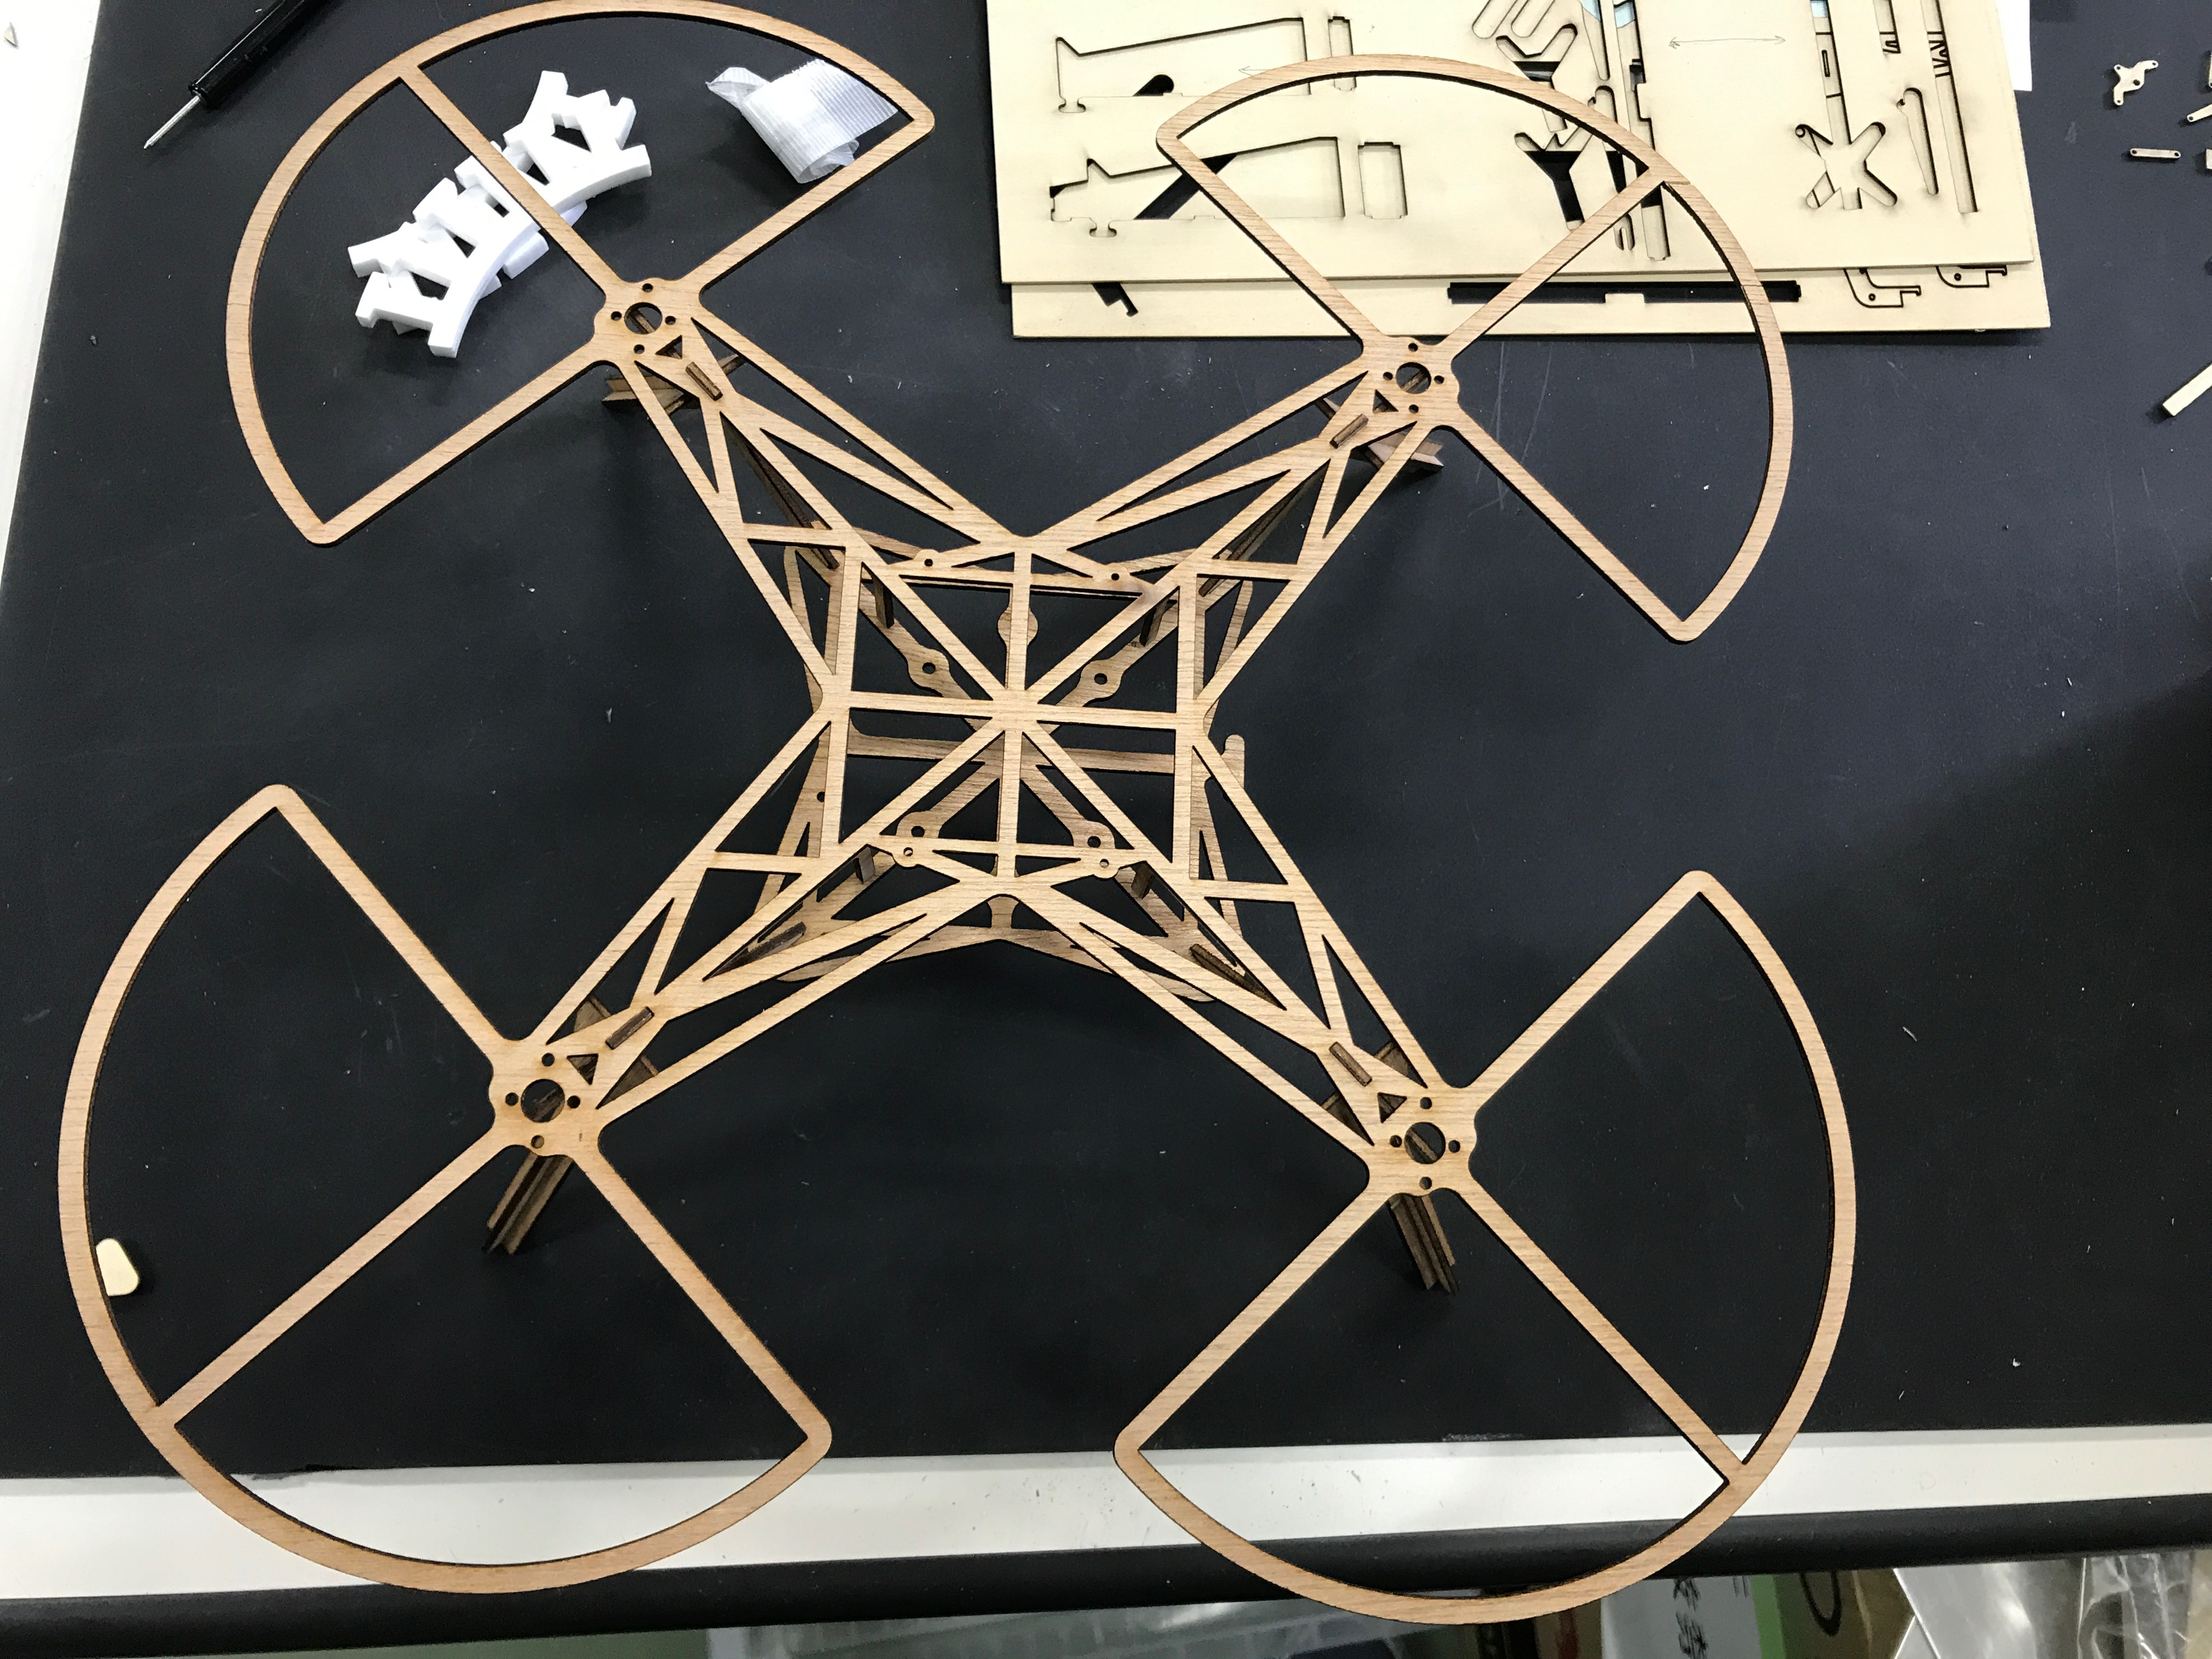
\includegraphics[width=80mm]{doutai.jpg}
    \end{center}
  \caption{胴体}
 \label{fig:doutai}
\end{figure}

\section{研究の目的}
大会出場時は飛行機の構成や原理など分かっていなかったため大会後、飛行機を設計するために知っておかないといけない構成や原理を理解するために簡単な飛行機を作り飛行機が飛行出来る原理の勉強を行いたいと考えていた.
しかし身近に原理を理解できる教材がなかったため,安く手に入りやすい材料を使い飛行原理を知らない人でも分かる教材の開発を作る事を目的としている.



\section{本論文の構成}
1章では,本研究の背景と簡略化した概要を示す.2章では飛行理論について,胴体の決定方法と絡めながら説明する.3章ではストロー飛行機の製作方法について述べる.4章では製作したストロー飛行機の飛行試験の結果について述べる.5章では本研究の結論を示す.